\chapter{Fonctions multiformes}
\section{L'application logarithme} 
L'application exponentielle complexe a été définie précédemment à
l'aide d'une série entière convergente dans $\mathbb{C}$. Il est
naturel de chercher une extension au plan complexe de son inverse,
l'application logarithme. Un complexe $z$ pouvant s'écrire sous la
forme $z = |z| \exp (i \theta)$ avec $\theta$ l'angle polaire associé à
$z$, on posera $log(z) = log(|z|) + i \theta$. L'application ainsi
définie ne possède malheureusement pas les bonnes propriétés que l'on
s'attendrait à obtenir. On notera en particulier qu'une discontinuité
se produit au franchissement de l'axe réel positif. Cependant, dans tout
domaine $U$ de $\mathbb{C}$ ayant une intersection nulle avec cet axe,
l'application logarithme est la fonction réciproque de l'exponentielle
complexe et est donc holomorphe dans $U$, sa dérivée étant~:
\[
log^\prime(z) = \frac{1}{z}
\]
On remarquera par ailleurs que si l'on pose de façon plus générale~:
\[
log(|z| \exp(i \theta)) = log(|z|) + i ( \theta + 2 k \pi)
\]
avec $k \in \mathbb{Z}$, l'application obtenue vérifie encore les
mêmes propriétés. On ne peut donc pas définir de façon univoque
l'application logarithme, mais ceci est possible seulement localement
(i.e. dans un domaine sans intersection avec $\mathbb{R}^+$) à
condition d'avoir fixé l'entier $k$. Par abus de langage, on appelera
application multiforme de coupure $\mathbb{R}^+$ une telle
application.
\section{Surfaces de Riemann}
Cette section est destinée à introduire un cadre formel permettant une
approche correcte des applications multiformes. Elle n'est cependant
pas nécessaire à la compréhension du reste du cours et peut être omise
en première lecture.

On rappelle qu'une application réelle ou complexe est dite analytique
sur un ouvert $U$ si elle est indéfiniment dérivable et égale à la
limite de son développement en série de Taylor en tout point de $U$. 
Soit $E$ un ensemble. On appelera carte de $E$ la donnée d'un triplet
$(U, \phi, F)$ avec $U$ partie de $E$, $F$ espace vectoriel réel ou
complexe et $\phi$ bijection de $U$ sur un ouvert de $F$. $U$ est
appelé domaine de la carte. Deux cartes $(U_1, \phi, F)$ et $(U_2,
\psi, F)$ sont compatibles si~:
\begin{itemize}
\item $\phi(U_1 \cap U_2)$ (resp. $\psi(U_1 \cap U_2)$) est un ouvert
de $F$.
\item L'application $\phi \circ \psi^{-1}$ (resp. $\psi \circ
\phi^{-1}$) de $\psi(U_1 \cap U_2)$ sur $\phi(U_1 \cap U_2)$ (resp. de
$\phi(U_1 \cap U_2)$ sur $\psi(U_1 \cap U_2)$) est analytique.
\end{itemize}
Enfin, on dira qie $E$ est une variété analytique si il existe une
famille $(U_i, \phi_i, F)_{i \in I}$ de  cartes deux à deux compatibles telle
que $\bigcup_{i \in I} U_i = E$.

Une variété analytique avec $F = \mathbb{C}$ est appelée surface de
Riemann. Une telle surface permet de généraliser la notion de graphe
d'une application. Soit en effet une application analytique $f :
\mathbb{C} \to \mathbb{C}$. La partie  $S \subset \mathbb{C}^2$ constituée des
couples de la forme $(z, f(z))$ est une surface de Riemann (prendre
comme carte l'application $\pi : \, S \to \mathbb{C}$ telle que
$\pi((z, f(z)) = z$). De façon générale, une surface de Riemann donne
localement une application analytique via les cartes, tout point de la
surface étant par définition dans le domaine d'une carte~: ceci permet
la définition des applications multiformes comme ensemble paramétré de
cartes d'une surface de Riemann. 

La figure \ref{Fi:fig4} montre partie imaginaire de  la surface de
Riemann associée à l'application $log$.
\begin{figure}[h]
\scalebox{.5}{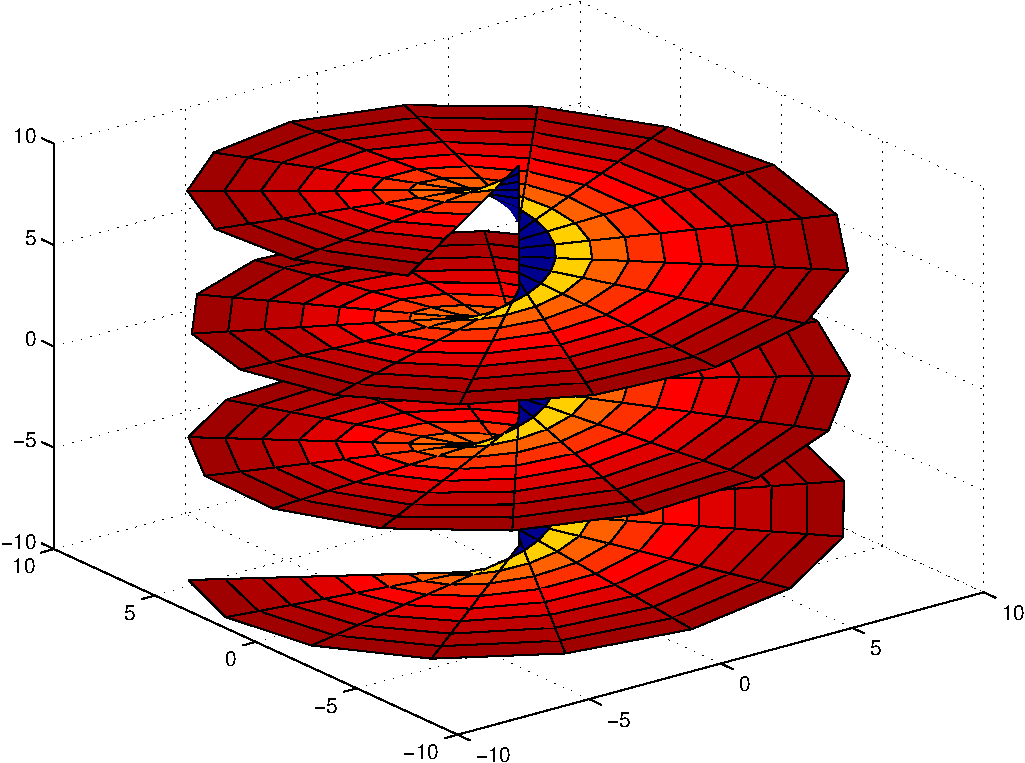
\includegraphics{images/fig4.pdf}}
\caption{Surface de Riemann de log}\label{Fi:fig4}
\end{figure}
\section{L'application racine n-ième}
Soit $n \in \mathbb{N}$.
Pour tout complexe $z = |z| \exp(i \theta)$, on pose $z^{1/n} = f_{n,k}(z) = 
|z|^{1/n} \exp i \left ( \frac{\theta+ 2 k \pi}{n}  
\right ) $ avec $k \in \mathbb{Z}$. Si l'on supprime le demi-axe réel
positif, l'application est holomorphe, sa dérivée étant~:
\[
f_{n,k}^\prime(z) = \frac{1}{n}{f_{n,k}(z)}{z}
\]

\leftline{\em Remarque}
Il est important de bien remarquer que l'on se place à $k$ fixé !

La surface de Riemann associée à la racine 3 ième est représentée
ci-dessous~:
\begin{figure}[h]
\scalebox{.5}{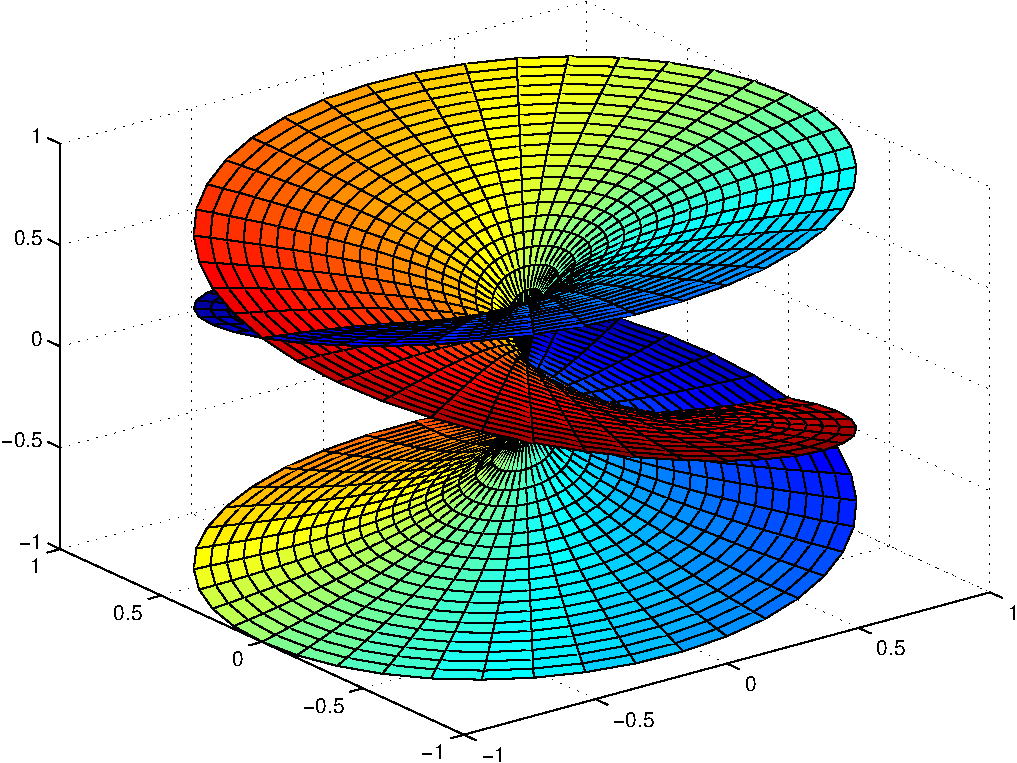
\includegraphics{images/fig5.pdf}}
\caption{Surface de Riemann de la racine 3 ième}\label{Fi:fig5}
\end{figure}
\section{L'application argument}
C'est l'application $f_k$ qui à $z = |z| \exp (i \theta)$ associe
$\theta + k 2 ^pi$. Ce n'est pas à proprement parler une application
multiforme, sa partie imaginaire étant nulle. On remarque par ailleurs
que cette application est simplement la partie imaginaire du
logarithme complexe. Par extension, on lui associera néanmoins une
surface de représentation dans $\mathbb{R^3}$~:
\begin{figure}[h]
\scalebox{.5}{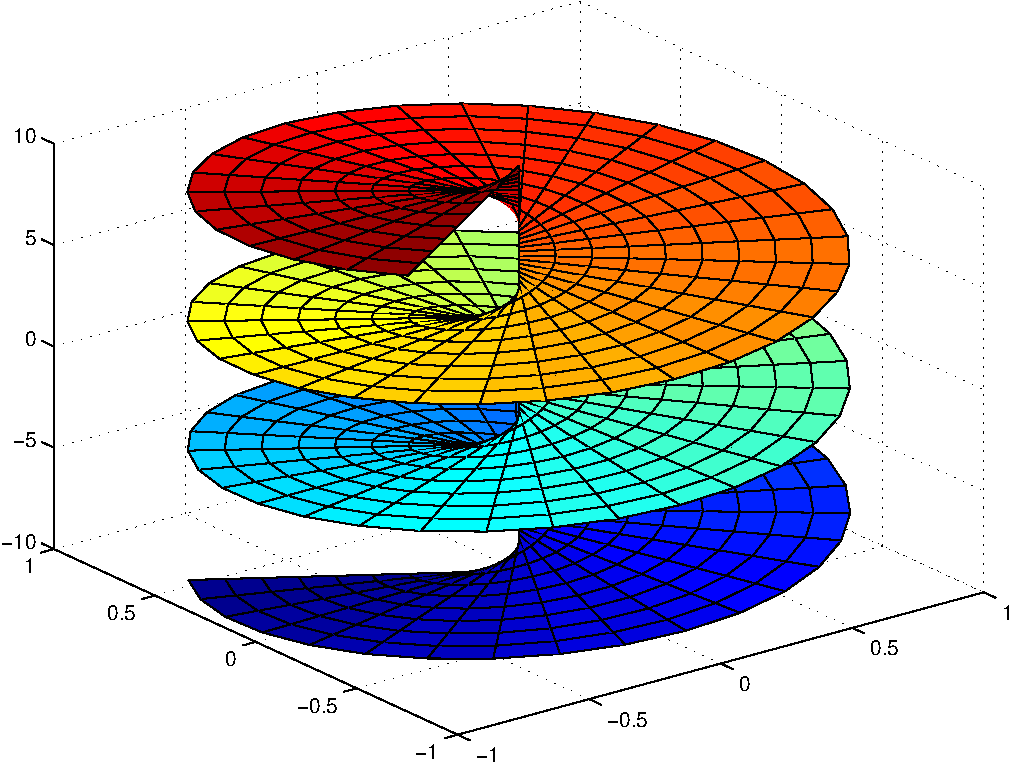
\includegraphics{images/fig3.pdf}}
\caption{Surface de représentation de arg}\label{Fi:fig3}
\end{figure}
\begin{exercice}
Calculer les intégrales~:
\[
I_1 = \int_0^{+\infty} \frac{x^2-1}{(x^2+1)^2}ln(x)dx
\]
\[
I_2 = \int_0^{+\infty} \frac{x^{a-1}}{1+x}dx, \, a \in ]0, 1[
\]
\end{exercice}